
\chapter{Documenting an API}
\label{ch:api}

\index{API (application programming interface)}
``\textbf{API}'' -- which historically stands for ``Application Programming
Interface'' -- is one of the dumber acronyms you'll encounter. And worse, it's
commonly used to mean two different things: (1) a set of classes (and their
methods) which a programmer could make use of in their own code, and (2) the
documentation describing those classes/methods.\footnote{By the way, the term
``API'' isn't used only for object-oriented software. One could write some
old-school procedural code (with functions and data structures, rather than
encapsulated classes and methods), describe it, and call that an API as well.}

In common lingo, people speak of ``programming to an API,'' which means
``writing some code which conforms to those documented classes.'' Every
time you've used an \texttt{ArrayList} or a \texttt{Scanner}, in fact, you
have been doing this. Instantiating such objects, calling methods on them, and
(importantly) reading the documentation at
\url{https://docs.oracle.com/javase/8/docs/api/} to find out how they
operate is all part of leveraging the built-in Java API for your own purposes.

These days, when we talk about using an API, we often mean writing code that
connects over the Internet to some publicly-available service or database of
information. Nearly every major Internet player these days -- Google, Youtube,
Instagram, Flickr, eBay, Twitter, Dropbox, Spotify, Amazon, \texttt{data.gov},
GeoDB cities, \textit{etc.} -- has a publicly-accessible API. This allows you
to write code (in any language) to connect to it and query it for information,
perform commands, make purchases, and so forth. Browse \url{dev.twitter.com} to
get an idea of the rich functionality available to anyone with the technical
savvy to understand and exploit an API.

It's an interconnected, collaborative world. Developers rarely write all the
code themselves anymore on a little isolated island. Instead, they share code
for others to use, and take advantage of what's been shared with them. If you
can figure out how to effectively do that, you've increased your programming
potential a hundredfold.

\section{The importance of good docs}

Now in order to make it possible for other developers to use the code you so
painstakingly wrote, it must be \textbf{documented} in a way that is clear,
complete, and unambiguous. To appreciate the importance of this, I want to
lead you in a thought experiment.

First, pretend you're back in the 1990's, a glorious time to be young and
alive. In particular, pretend that \textit{GPS and cell phones are not yet
commonly available.} (Believe it or not, this was true in the recent past.)

\index{party}
\index{Biff}
\index{Filbert}
Let's suppose it's Friday night, and you're going to a party at the apartment
of your acquaintance Biff. Biff lives up in North Stafford, and you've never
been to his place before. Luckily, your close friend Filbert is also going to
the party, and he's been to Biff's on many occasions. You're picking him up at
8pm.

Consider the following two scenarios.

\begin{description}

\item[Scenario A:] You'll pick up Filbert (and possibly one or two others), and
drive together to Biff's apartment.

\item[Scenario B:] Filbert calls you at the last minute and says that he's
getting a ride with somebody else. He gives you \textit{written directions} to
Biff's, however, so that you can get to the party on your own.

\end{description}

My question: in which of the above two scenarios are you \textit{more} likely
to successfully arrive at the party without getting lost? Or are both cases
equally likely?

The careless thinker might at first conclude that the two cases are equally
likely. After all, they both depend on Filbert's knowledge of how to get to
Biff's. In one case, Filbert's verbalizing the directions as you drive, and in
the other case, he's laying them all out for you in advance. But
theoretically, as long as Filbert knows how to get there, you'll be successful
in both scenarios.

Theoretically. But in the real world, as everyone knows, it usually doesn't
work like that. In scenario A, with Filbert in the passenger seat, you have the
chance to interactively ask about every intersection and every turn. But in
scenario B, \textit{Filbert had to specify everything perfectly in advance.}
He had to describe the route with no errors, since there would be no chance to
make corrections en route. He had to anticipate every question you might have,
since he wouldn't be there to answer them. That's a lot of pressure on Filbert
to give good directions.

Consider the following very realistic possibilities:

\begin{itemize}
\itemsep.1em

\item Filbert wrote ``left'' when he meant ``right'' in step 3 of the directions
because he's human.

\item Filbert just plain forgot step 5 of the directions because he's human.

\item When he wrote, ``turn left at the next opportunity,'' he meant ``at the
next \textit{intersection},'' and assumed that would be obvious to you.
However, you (quite naturally) thought he meant ``the very next possible
left,'' which was down a side road.

\item A road is closed, or there's a traffic jam, and you need to improvise
in order to make it to the party on time.

\item \textit{Etc.}

\end{itemize}

You can think of a dozen more. In all these cases, having Filbert with you in
the car allows you to clarify ambiguities, fill in omissions, ask questions as
they arise, and change course in response to unexpected circumstances. With
the written directions, you have none of those options. Put another way,
Filbert isn't even at your disposal in Scenario B: your only asset is
Filbert's brain dump, as he was conceiving it at 6:13pm.

And by the way: most people are pretty bad at giving directions.

\subsection{Collaborating with someone you'll never meet}

In case the above analogy isn't plain, Scenario A corresponds to a software
development team where your teammates are just down the hall. They're just an
email or a Slack away. You can ask questions, report bugs, or even request
alterations as the need arises. The pressure is off, as far as documentation
is concerned. In fact, why even bother trying to document everything
exhaustively in advance, if your teammates can ask focused questions in real
time?

Scenario B corresponds to you using a public API. The instructions written by
a developer you will never meet are \textit{your one and only chance} to
comprehend how to use the thing. Those instructions had better be darned good,
because there is no chance to ask questions on the road. They'd better clearly
and exhaustively contain \textit{everything} you're likely to want to know.

By the way: most people are pretty bad at writing clear and complete
documentation. The good news is that it's possible to improve this through
discipline, practice, and painstaking effort.

\section{JavaDoc: mechanics}

\index{javadoc@\texttt{javadoc}}
One of Java's supplementary (but in retrospect, killer) features was the
\texttt{javadoc} utility shipped with the JDK. The idea behind JavaDoc was to
combine two previously incompatible aspects of code documentation. The key
question is: where should the documentation be kept?

On the one hand, it seems that the English text describing how to use a
software component (like a class, method, or package) ought to be maintained
right alongside the code itself, in the source file. This promotes keeping the
code and the docs in sync.

On the other hand, there are clearly many advantages to presenting the
documentation in a rich, interactive, point-and-click hypertext format. Then
the user can browse it non-linearly, read it with pretty formatting, avoid
having to step around the code itself to read the next bit of documentation,
\textit{etc.} 

So we seem to have two conflicting desires: to keep the documentation close to
(and embedded in) the code, and to author it in a more flexible (and ideally,
web-browser-accessible) way outside the code.

\index{java file@\texttt{.java} file}
JavaDoc's innovation was to say: ``go ahead and store the documentation in the
\texttt{.java} files themselves, to promote consistency. But we'll create a
separate tool that can examine the \texttt{.java} files and extract the
documentation portions. The tool will then assemble those into a mini-website
that other programmers can conveniently browse.''

To accomplish this, we use a special syntax to denote ``JavaDoc comments.''
Recall that one style of comment in Java is the multi-liner:

\vspace{-.11in}
\begin{Verbatim}[fontsize=\footnotesize,samepage=true,frame=none]
  /*
   * This is a regular Java comment, and will be ignored by javac.
   */
\end{Verbatim}
\vspace{-.11in}

JavaDoc comments are the same, except that they have a \textit{double}
asterisk at the beginning:

\vspace{-.11in}
\begin{Verbatim}[fontsize=\footnotesize,samepage=true,frame=none]
  /**
   * This is a special JavaDoc comment, which will be ignored by
   * javac, but will be extracted by javadoc.
   */
\end{Verbatim}
\vspace{-.11in}

You can place JavaDoc comments in three places:

\begin{itemize}
\itemsep.1em

\item Immediately before a class definition, to provide a description of that
class, and hints as to its usage.

\item Immediately before a method definition, to describe what the method
does, how to call it, and what will happen in exceptional conditions.

\index{package.html@\texttt{package.html}}
\item In a special file called ``\texttt{package.html}'', which will be placed
in the source directory for a package, if you're using Java packages.

\end{itemize}

The \texttt{javadoc} utility will automatically identify and extract the
English text stored in JavaDoc comments in any of these three places, and
assemble them into HTML files in the appropriate way.

\subsection{Markup and tags}

There are also a couple of cosmetic options you can take advantage of in
JavaDoc comments. First of all, any valid HTML tag can be used directly in the
comment, and will be formatted appropriately in the final mini-website. If
you're familiar with HTML tags like ``\texttt{$<$b$>$}'' (for boldface),
``\texttt{$<$tt$>$}'' (for a monospace, typewriter font) or
``\texttt{$<$ul$>$}'' and ``\texttt{$<$li$>$}'' (for bulleted lists), you can
use them to style your text.

Second, there are special tags called ``JavaDoc tags'' that can be used to set
apart certain meta-information and put them in a special place in the final
HTML product. The most important ones are shown in Figure~\ref{fig:taglist},
though there are others. Each development team acquires their own culture,
policies, and procedures that call for different pieces of information to be
highlighted.

% https://tex.stackexchange.com/questions/343028/vertical-centering-of-all-columns-in-tabularx-environment
\renewcommand\tabularxcolumn[1]{m{#1}}

\begin{figure}[ht]
\centering
\scriptsize
\begin{tabularx}{\textwidth}{|c|c|X|}
\hline
Tag/syntax & Location & Purpose\\

\hline
\hline

\index{author tag@\texttt{"@author} tag}
\texttt{@author} \ Jezebel & class & 
The primary or original author of the class. Using the first name, username, or
initials of the author are common choices.\\

\hline

\index{param tag@\texttt{"@param} tag}
\texttt{@param} \ \texttt{name} \ description & method & 
What one of the arguments to the method means.
``\texttt{name}'' is either the name or the type of argument.
``description'' should begin with a lower-case letter
and end with a period.\\

\hline

\index{return tag@\texttt{"@return} tag}
\texttt{@return} \ description & method & 
How the return value of the method should be
interpreted. ``description'' should begin with a
lower-case letter and end with a period.\\

\hline

\index{throws tag@\texttt{"@throws} tag}
\texttt{@throws} \ type \ description & method & 
What type of exception might be thrown from the
method and how it should be interpreted.
``description'' should begin with the word ``if'' and
end with a period.\\

\hline
\index{link tag@\texttt{"@link} tag}
\texttt{\{@link className\}} & anywhere &
Create a clickable hyperlink to the class named.\\

\hline

\texttt{\{@link className\#method\}} & anywhere &
Create a clickable hyperlink to the method named.\\

\hline

\index{deprecated tag@\texttt{"@deprecated} tag}
\texttt{@deprecated} \ explanation &
\makecell{class / \\ method} & 
Mark this class or method as old and not to be used
by new code. (Still supported temporarily for older
code, but intended to be phased out.)\\

\hline

\end{tabularx}
\vspace{.1in}
\caption{Some commonly-used JavaDoc tags, and their meanings.}
\label{fig:taglist}
\end{figure}
\normalsize

A representative example showing many of these tags is in
Figure~\ref{fig:javadocTags}, the HTML for which appears in
Figure~\ref{fig:javadocApi}.

\index{ballplayer@\texttt{Ballplayer}}
\begin{figure}
\begin{Verbatim}[fontsize=\scriptsize,samepage=true,frame=single]
/**
 * A <tt>Ballplayer</tt> represents a historical baseball player and
 * the composite statistics over his career. Each <tt>Ballplayer</tt>
 * object is associated with one {@link Team} even if he played for
 * multiple teams in his actual career.
 * @author SD
 */
public class Ballplayer {
    ...
    /**
     * Constructs a new <tt>Ballplayer</tt> object with "empty" stats
     *   (<i>i.e.</i>, all set to their initial, default values.)
     * @param name the real (no nicknames) first and last name of the
     *   player.
     * @param uni the most well-known uniform number he played under.
     * @param team the mascot name (not city) of the {@link Team} he
     *   is most commonly associated with.
     * @throws NoTeamException if the <tt>team</tt> parameter does not
     *   correspond to the mascot name of any known {@link Team}.
     */
    public Ballplayer(String name, int uni, String team)
        throws NoTeamException {
        ...
    }
    
    /**
     * Returns the player's career batting average, measured as total
     *   hits divided by total "at bats." If the number of "at bats"
     *   is zero, returns 0.0 rather than give a divide-by-zero error.
     * @deprecated This method should be eschewed in favor of more
     *   recent stats such as {@link Ballplayer#getOnBasePercentage}
     *   and {@link Ballplayer#getSluggingPercentage}.
     * @return the batting average on a 0.0-to-1.0 scale.
     */
    public double getBattingAvg() {
        ...
    }
}
\end{Verbatim}

\caption{HTML and JavaDoc tags in action.}
\label{fig:javadocTags}
\end{figure}


\subsection{Generating the mini-website}

\index{javadoc@\texttt{javadoc}}
To actually generate the HTML in Figure~\ref{fig:javadocApi}, you'll need to
run the \texttt{javadoc} command with some options. Generally, if I'm running
on a Google Cloud instance, this is how I run it:

\begin{Verbatim}[fontsize=\small,samepage=true,frame=none]
$ sudo javadoc -d /var/www/html -author *.java
\end{Verbatim}

\index{sudo@\texttt{sudo}}
\index{root user@\texttt{root} user}
The word ``\texttt{sudo}'' at the start of this sentence means ``please allow
me to execute the following command as the \textbf{root} user of the system'';
\textit{i.e.}, the super user who has all privileges. The reason this is
necessary is that the directory \texttt{/var/www/html}, which this command
says to write content in, is by default not writeable by ordinary mortals. You
have to temporarily become Superman in order to write to it, which will
require typing your password to confirm you're really Clark Kent.

\index{option}
The ``\texttt{-d /var/www/html}'' bit is a command option with a parameter. The
\texttt{-d} stands for ``directory'' and it says that the HTML that
\texttt{javadoc} generates should be written to this directory. It's a
system-specific thing; on Debian Linux (which I install on Google Cloud) this
is the directory that Apache Web Server will look in to serve up content to
browsers that connect to it. (More on that in a moment.) In other contexts,
like if you have a user directory on a shared machine that you don't have
control over, you can often substitute something like ``\texttt{-d
/home/yourusername/public\_html}'' which will write the content to your
account's own directory for hosting HTML content to the world.

\index{public@\texttt{public}}
\index{private@\texttt{private}}
The ``\texttt{-author}'' part of the command says ``yes, please \textit{do}
extract \texttt{@author} information and include it in the HTML. (The default
is to not do that, which I've never understood.) Semi-related: by default
\texttt{javadoc} only includes the \textbf{public} classes and methods in the
HTML it generates, since JavaDoc is normally used to document public APIs.
Sometimes there are reasons to produce JavaDoc content for \textit{everything}
in the class files -- private, public, or anything else -- and to do this you
merely need to include a ``\texttt{-private}'' option here as well.

\index{java file@\texttt{.java} file}
Finally, the ``\texttt{*.java}'' means to generate HTML for all the Java source
files in the current directory. If you're using packages, you can instead
replace ``\texttt{*.java}'' with a sequence of fully-specified package names
that can be located via the \texttt{CLASSPATH} variable. Note that you
do have to tell \texttt{javadoc} to generate the \textit{entire} mini-website
at once; if you make just a change or two to one \texttt{.java} file, you
can't just regenerate the HTML for that one because then the entire
mini-website will consist of nothing \textit{but} that one class.

\subsubsection{Starting the Web server and connecting}

\index{Apache Web Server}
After all the JavaDoc's mini-website content has been generated, you can
access it via your browser. You can find out whether Apache Web Server is
running by typing:

\begin{Verbatim}[fontsize=\small,samepage=true,frame=none]
$ sudo systemctl status apache2
\end{Verbatim}

at the command line. If it gives a message like ``whoa, apache2 not
installed,'' then you'll need to install it via:

\begin{Verbatim}[fontsize=\small,samepage=true,frame=none]
$ sudo apt install apache2
\end{Verbatim}

If it says it's not currently running, then you'll need to start it via:

\begin{Verbatim}[fontsize=\small,samepage=true,frame=none]
$ sudo systemctl start apache2
\end{Verbatim}

\index{IP address}
Lastly, when this seems to be working, figure out what the external IP address
is of your machine (it'll be four numbers, each in the range 0-255, set apart
by periods; for example, 35.237.255.14). Then, you can point your browser to
\url{http://thatIPAddress} and you should be able to see your
prettily-formatted HTML website like in Figure~\ref{fig:javadocApi}.

\subsubsection{Firewall settings}

\index{firewall settings (Google Cloud)}
If you can't reach your JavaDoc site via the above URL, your problem might be
that your Google Cloud firewall is blocking the traffic. At the time of this
writing, here's how to fix that problem:

\begin{compactenum}

\item Go to \texttt{https://console.cloud.google.com/networking/}\\\texttt{firewalls/list}.
\item Click ``Create firewall rule.''
\item Give it a name like ``\texttt{allowhttp}''.
\item Choose ``All instances in the network'' from the ``Targets'' drop-down.
\item Make sure direction is ``Ingress'' and action is ``Allow''.
\item For ``Source IP ranges'' put ``\texttt{0.0.0.0/0}''.
\item Click TCP under ``Specified protocols and ports'', and put in \texttt{80}.
\item Click ``Create'' to create the rule.
\end{compactenum}



\begin{figure}
\centering
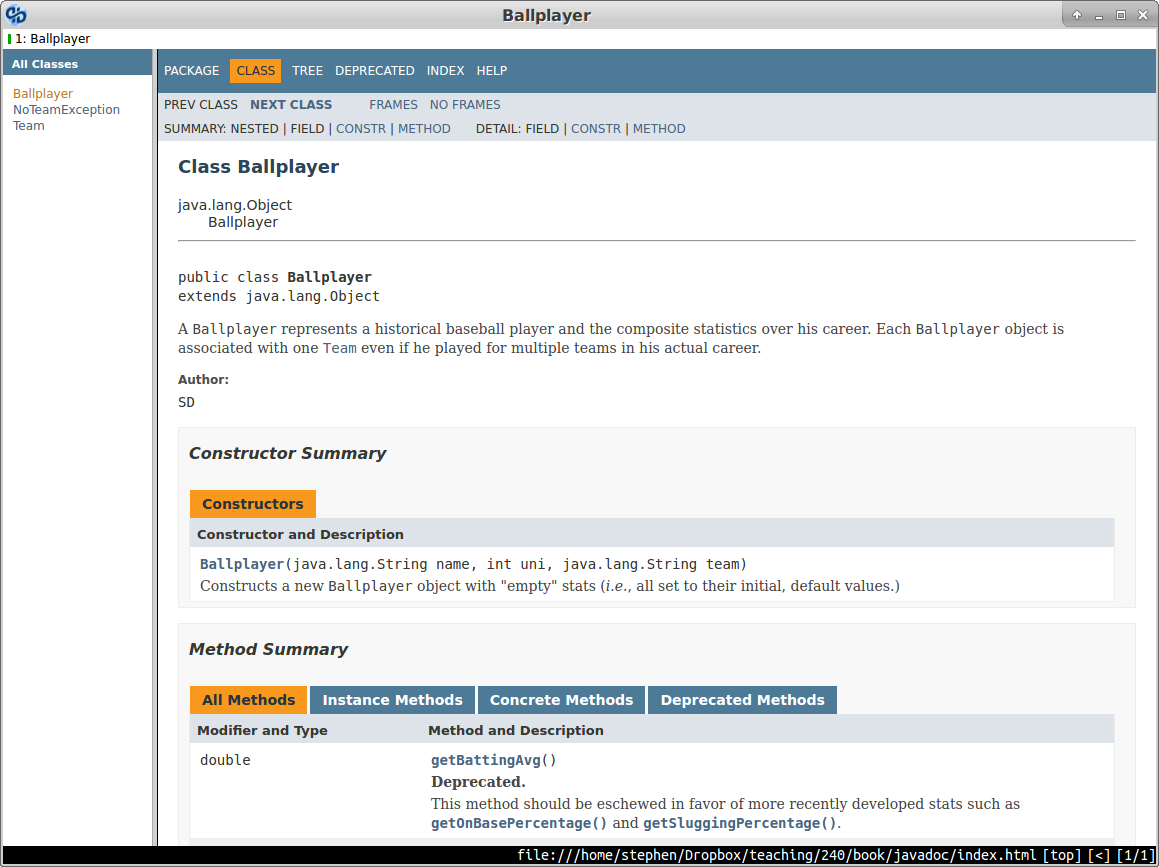
\includegraphics[width=1\textwidth]{javadoc1.png}

\vspace{.2in}

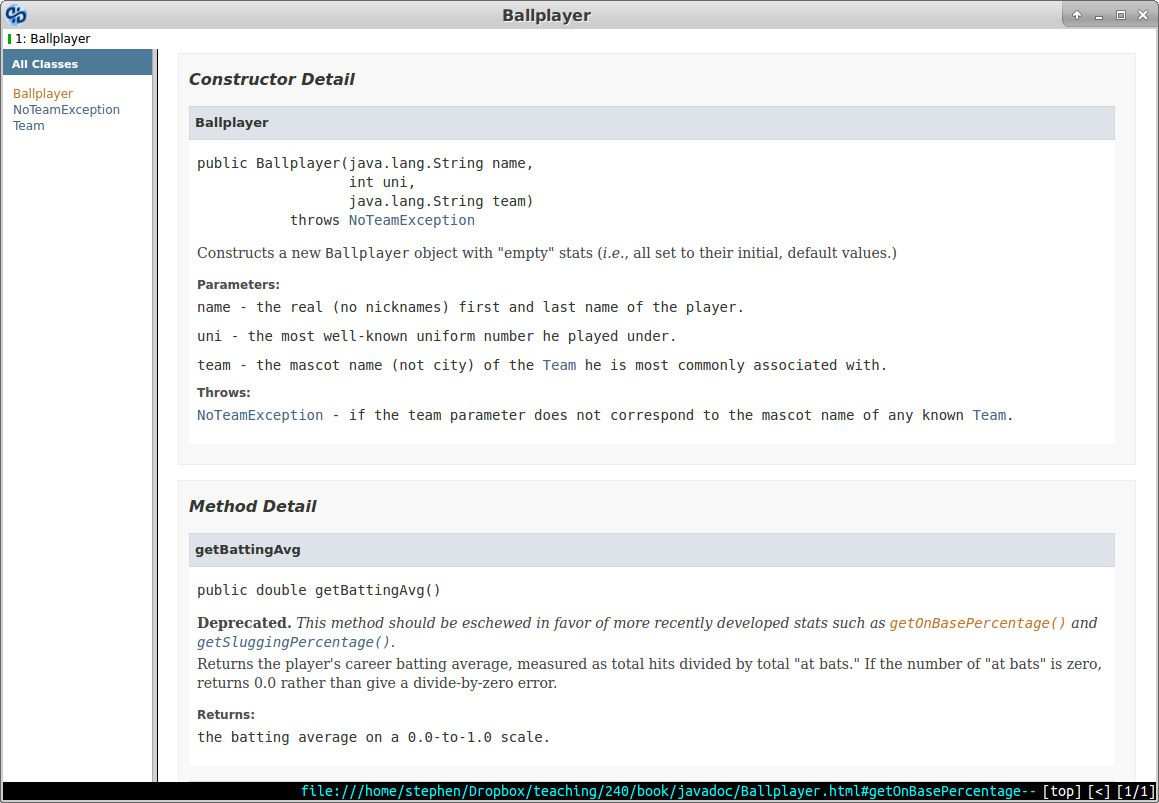
\includegraphics[width=1\textwidth]{javadoc2.png}

\vspace{.2in}

\caption{The generated HTML for the code in Figure~\ref{fig:javadocTags}.}
\label{fig:javadocApi}
\end{figure}


\section{JavaDoc: content}

Okay, so that's all the minutiae of how to get the JavaDoc syntax right and
generate the website. You have to know this, but it actually isn't the
important part. The truly important question in all this is less-easily
defined: how to actually write quality documentation that will communicate
effectively to programmers I may never meet?

\pagebreak
The answer is at once super simple and extremely nuanced. Here is the one and
only rule that should guide your API documentation process:

\definecolor{shadecolor}{rgb}{.9,.9,1}
\begin{shaded}
\begin{quote}

\textbf{\textsf{``Put yourself in the shoes of a Java developer who has never
seen your code before. Write whatever that person would need to know in order
to use your code properly.''}}

\end{quote}
\end{shaded}

You might be surprised how much students (and professionals) struggle
implementing this advice. It turns out that the human brain has a very
difficult time envisioning what it's like to \textit{not already know}
something. ``Putting yourself in someone else's shoes'' just doesn't come
naturally, it seems. Nevertheless, you \textit{must} do it, otherwise your
documentation will be pretty useless.\footnote{As an aside, this same mantra
-- ``put yourself in the shoes of someone who doesn't already know'' -- is the
essence of another common activity: \textit{teaching}. With few exceptions,
I've discovered that a good teacher is one who can mentally put themselves in
the shoes of their students, and remember what it was like to not already know
the material. Conversely, bad teachers are inevitably poor at this exact
skill, which is why it can sometimes seem as if they're assuming you already
possess the knowledge before they began to teach it!}


\subsection{Class documentation}

Classes are the easier of the two main components (the other being methods) to
write JavaDoc for. That's because the purpose of class JavaDoc is mostly to
orient the reader to the class's purpose and what it collaborates with. Still,
it's certainly possible to leave important information undefined or ambiguous.

\index{team@\texttt{Team}}
Let's take a look a bad attempt to document the \texttt{Team} class from the
baseball simulator example, followed by some better ones.

\pagebreak
First (bad) attempt:
\vspace{-.15in}
\begin{Verbatim}[fontsize=\footnotesize,samepage=true,frame=single]
/**
 * A <tt>Team</tt> represents a group of {@link Ballplayer}s
 * who play baseball together.
 */
public class Team {
    ...
}
\end{Verbatim}
\vspace{-.1in}

This JavaDoc succinctly sums up what the \texttt{Team} class is for, but I
claim it leaves out at least two important pieces of \textit{non-obvious}
information. ``Non-obvious'' is the key word here: the stuff that would be
obvious to a reader isn't particularly important to document. It's the things
that \textit{aren't} clear that deserve attention.

One thing this JavaDoc is missing is the motivating \textit{reason} for using
the class. A fellow developer might read this and say, ``okay, a \texttt{Team}
is a group of \texttt{Ballplayer}s, but if that's all it is, I'll just use
\texttt{ArrayList} instead, since I'm more familiar with it.'' It's a fair
point: our JavaDoc hasn't made the sale as to why it's worth using.

\index{simulator@\texttt{Simulator}}
Okay, so why \textit{is} it worth using? At least two reasons are (1) it can
be used as input to the \texttt{Simulator} class, in order to simulate a
virtual ballgame, and (2) it has useful methods on it that provide summary
statistics for the entire team. So let's say that:

\smallskip
Second (better) attempt:
\vspace{-.15in}
\begin{Verbatim}[fontsize=\scriptsize,samepage=true,frame=single]
/**
 * A <tt>Team</tt> represents a group of {@link Ballplayer}s who play
 * baseball together, and can compute summary statistics about the
 * group's past performance. Two <tt>Team</tt> objects are required to
 * run a single-game simulation (see {@link Simulator#simSingleGame}.)
 * Methods like {@link Team#getTeamBattingAverage()} and
 * {@link Team#getWonLossRecord()} can be called to get aggregate
 * information about the team's performance.
 */
public class Team {
    ...
}
\end{Verbatim}

Better. And now for the second thing I found missing. One crucial aspect of
documentation to include -- and one that is easily overlooked -- is the
\textit{assumptions} the developer was making when she wrote the class, but
which a user of the class might not make. In this case, a glaring question is:
``can a \texttt{Ballplayer} be a member of more than one \texttt{Team}?'' Frank
Robinson, for instance, was a Hall of Fame outfielder for both the Cincinnati
Reds and the Baltimore Orioles. What would happen if I attempted to add him to
two different \texttt{Team} objects? Is it perfectly okay? Is it forbidden,
but not checked by the code? Or will adding him to the second object trigger a
run-time exception?

It's imperative that we know, because all three of the above behaviors are
reasonable. In order to use this \texttt{Team} class, we need to know which
one is the true behavior.

So let's add that information in, together with an author tag, and call it
done (at least for now):

\smallskip
Final attempt:
\vspace{-.1in}
\begin{Verbatim}[fontsize=\scriptsize,samepage=true,frame=single]
/**
 * <p>A <tt>Team</tt> represents a group of {@link Ballplayer}s who
 * play baseball together, and can compute summary statistics about
 * the group's past performance. Two <tt>Team</tt> objects are required
 * to run a one-game simulation (see {@link Simulator#simSingleGame}.)
 * Methods like {@link Team#getTeamBattingAverage()} and
 * {@link Team#getWonLossRecord()} can be called to get aggregate
 * information about the team's performance.</p>
 * 
 * Note that a <tt>Ballplayer</tt> can be a member of <i>any number</i>
 * of teams. (This will happen if a player was traded during his
 * career, for instance.) In this case, the summary statistics for each
 * <tt>Team</tt>, and its performance in a simulation, will take place
 * as though that player's entire career stats applied to <i>each</i>
 * of his teams.
 *
 * @author Stephen
 */
public class Team {
    ...
}
\end{Verbatim}

\pagebreak
\index{Stephen}
\index{Henderson, Rickey}
Apparently, \texttt{Stephen} has decided to write the \texttt{Team} code to
deliberately \textit{allow} a ballplayer to be a member of more than one team.
This JavaDoc also spells out a possibly unexpected caveat of this decision:
the system doesn't separately keep track of which stats a player accumulated
on which of his teams, but simply lumps them all together in a single
\texttt{Ballplayer}. This has an important impact on what to expect from the
simulator's behavior, if (for instance) a player was traded late in his
career. If you have an aging Ricky Henderson on your L.A. Dodgers squad, that
team is going to benefit from \textit{all} Ricky's legendary base-stealing,
even though almost all of it occurred with different teams earlier in his
career.

The point is that this clarifies an important case that perhaps wasn't obvious
at first. In general, it's really easy to think of only the ``sunny day''
scenarios, and to write the documentation describing what is normally pretty
obvious anyway. It's harder to step out of the box and recognize what cases
\textit{aren't} so obvious -- in this example, the multiple-team-players
question -- and give the user of the class guidance on what to expect.


\subsection{Method documentation}

Method documentation is a higher-stakes affair than class documentation,
simply because there are more details to remember and to get right. It's not
often that a fellow developer gets off in the weeds about what a class is even
used for; but it's not rare for them to code to a method incorrectly because
the JavaDoc is spurious or misleading.

\index{getOPS@\texttt{.getOPS()}}
Taking again the baseball example, let's look a bad attempt to document the
\texttt{.getOPS()} method.

First attempt:
\vspace{-.15in}
\begin{Verbatim}[fontsize=\footnotesize,samepage=true,frame=single]
    /**
     * Return the player's OPS.
     */
    public double getOPS() {
        ...
\end{Verbatim}

This is an example of wasting time typing. The programmer might as well have
typed nothing at all, since ``returning'' was implied in ``\texttt{get}...'' and
\texttt{OPS} remains undefined. Let's try again.

\smallskip
Second attempt:
\vspace{-.1in}
\begin{Verbatim}[fontsize=\footnotesize,samepage=true,frame=single]
    /**
     * Return the player's career OPS (On-base-plus-slugging)
     * statistic, defined as the player's on-base percentage
     * plus his slugging percentage.
     */
    public double getOPS() {
        ...
\end{Verbatim}

This is much more useful, at least, since it defines for a reader who may not
be familiar with the more advanced Sabermetric stats what ``OPS'' even is.
Still a few things missing, though. For one, the on-base percentage and
slugging percentage are both defined on a 0.0-to-1.0 scale rather than a
0-to-100 scale, and so ``percentage'' is a very misleading (incorrect,
actually) word. We don't want to move away from standard baseball
conventions, so we'll keep the terms but then make the scale clear in a note
in the JavaDoc.

\label{batting average}
Speaking of standard baseball conventions...all the stats like batting
average, slugging percentage, OPS, \textit{etc.} are traditionally reported to
exactly \textit{three} decimal places. We say ``Simpson is hitting .325,'' not
``Simpson is hitting .3257886442.'' Another question that arises, then, is: do
methods like \texttt{.getBattingAvg()} and \texttt{.getOPS()} return a figure
rounded to the three decimal places of convention, or do they return
hits-divided-by-at-bats (or whatever) with all possible precision? One can see
advantages to doing it either way; the point here is that the JavaDoc must
specify which it is.

Whether to document here what ``on-base percentage'' and ``slugging percentage''
themselves are is a judgment call. If there are other methods on the
\texttt{Ballplayer} class specifically for those two stats, then it's probably
better to link to them in the \texttt{.getOPS()} JavaDoc rather than duplicate
the text.

\label{corner case}
Finally, you always have to ask yourself ``what corner cases are there?'' What
scenarios might unfold that are unusual and need special treatment? Here, the
important one turns out to be a ballplayer \textit{with no at-bats.} In this
case, both his on-base percentage and his slugging percentage will have a
denominator of \textit{zero}, which is an illegal mathematical operation.
(``Zero hits divided by zero at bats'' is not zero, but undefined.)
Traditionally, players with no batting chances are reported as having a .000
batting average, slugging percentage, on-base percentage, \textit{etc.}, so it
makes sense for our method to do that here. When it does, though, it's
strictly speaking going beyond the definition of ``successes divided by
attempts'' that all these averages are based on.

Answering all these questions adequately, then, leads to this JavaDoc:

Final attempt:
\vspace{-.15in}
\begin{Verbatim}[fontsize=\scriptsize,samepage=true,frame=single]
/**
 * Return the player's career OPS (On-base-plus-slugging) statistic,
 * defined as the player's on-base percentage plus his slugging 
 * percentage. On-base "percentage" is computed on a 0-to-1 scale,
 * not 0-to-100 (and slugging "percentage" is similar, though it can
 * be as high as 4.0 (all home runs)), so this method's return value
 * should not be interpreted as a "percentage" either.
 * 
 * Although OPS is typically reported to three decimal places, this
 * method will not perform any rounding to ensure that; full precision
 * to as many decimal places as the system allows will be reported.
 *
 * For <tt>Ballplayer</tt>s with zero plate appearances, this method
 * will return 0, not a divide-by-zero error.
 *
 * @return the player's career OPS statistic.
 */
public double getOPS() {
    ...
\end{Verbatim}

\index{return tag@\texttt{"@return} tag}
You may be thinking that the \texttt{@return} line at the end doesn't really
add anything useful. You would be correct. I included it only for
completeness; in general, it's fine to leave out redundant information. Some
developers like to use the ``\texttt{@}'' tags religiously, while others like
to put key information in the running text of the JavaDoc. This is a stylistic
choice, and either way is okay. The crucial thing is that \textit{the
information has to be present somewhere.}

You also may be thinking that it's tough to come up with all this stuff. You
would also be correct about that. Once you see me explain that ``zero plate
appearances'' is a non-obvious special case, or that it's an open question
whether the method would round to three decimal places, you can probably say
``oh yeah, we'd better mention that detail.'' Of course, the challenge is to
recognize what those details are \textit{before} they're pointed out to you.

Honestly, I can think of no way to make this easier other than (1) practice,
and (2) really truly trying to put yourself in the mindset of a new developer.
It's hard to pretend you're someone else -- and to momentarily, deliberately
forget what you know -- but it's not impossible. And as I said earlier, it's
really the key to communication of all kinds.

\subsubsection{Important: \textit{don't} mention implementation!}

The most common error (and it is indeed an \textit{error}) that I see students
making when writing their method-level documentation is including
implementation details in their description.

For instance, suppose our \texttt{Team} class had a method called
\texttt{.add()} which could add a \texttt{Ballplayer} to the team. Here's a
very common, but also very wrong, way to write its JavaDoc:

\vspace{-.15in}
\begin{Verbatim}[fontsize=\scriptsize,samepage=true,frame=single]
    /**
     * !WRONG! Include a new {@link Ballplayer} object in this
     * <tt>Team</tt> by adding it to this object's "players"
     * <tt>ArrayList</tt>.
     */
    public void add(Ballplayer bp) {
        ...
\end{Verbatim}

\index{encapsulation}

Do you see the problem? If you've learned anything in this book, I hope you do.
\textit{Our documentation has seriously violated encapsulation here}, and of
course encapsulation is the whole freaking point of OOP.

Specifically, \textit{users} of the \texttt{Team} class should neither know nor
care \textit{how} the \texttt{.add()} method does its work. They should neither
know nor care whether there's an \texttt{ArrayList}, or anything else,
involved, let alone the name of a specific instance variable (which is
``\texttt{players},'' apparently). They should only be told \textit{what} the
method does -- what behavior to expect when it's called.

There are two reasons for this. One, that implementation info is simply
irrelevant to clients. if I'm writing code that instantiates and uses
\texttt{Team} objects, I don't need to know what its instance variables are, or
anything else under the hood. It's a distraction. Two, if we did reveal that
information, we would be loudly advertising something that is subject to future
change. Suppose we decided to store a \texttt{Team}'s \texttt{Ballplayer}s in a
\texttt{Hashtable} instead of an \texttt{ArrayList}, or in some other object
entirely? It would sure be awkward if we had baked into our public
documentation the statement about ``a \texttt{players} \texttt{ArrayList}''!

Here's a correct version:

\vspace{-.15in}
\begin{Verbatim}[fontsize=\scriptsize,samepage=true,frame=single]
    /**
     * !RIGHT! Add a new {@link Ballplayer} to this <tt>Team</tt>,
     * which will thereafter use it in single-game simulations and
     * include it in its aggregate statistics.
     *
     * Note that a <tt>Ballplayer</tt> can be a member of
     * <i>multiple</i> <tt>Team</tt>s, so calling this method on one
     * <tt>Team</tt> will not remove the player from any others.
     *
     * If the <tt>Ballplayer</tt> is already a member of this
     * <tt>Team</tt>, this method will have no effect.
     * 
     * <tt>Ballplayer</tt>s added to a <tt>Team</tt> can be later
     * removed from it via the {link Team#remove} method.
     */
    public void add(Ballplayer bp) {
        ...
\end{Verbatim}

\index{underwear drawer}

The documentation is now chock-full of important information that a client of
the \texttt{Team} class would need to know, and shows off nothing in the
underwear drawer. The general rule here is: if something's \texttt{private}
(which certainly includes instance variables) \textit{don't} mention it in the
JavaDoc.

\medskip

\index{what vs. how@``what'' vs.~``how''}

One other similar rule is this: don't make your method-level JavaDoc a
step-by-step narration of what the method's code is going to look like. Again,
the purpose of the JavaDoc is to specify \textit{what}, not \textit{how}.

\section[How to lose a battle]{How to lose a battle through bad documentation}

\index{Burnside, Ambrose}
\index{Battle of Fredericksburg}
\index{Civil War}
\index{Franklin, William}
\index{Lincoln, Abraham}
I'll close this chapter -- and book -- with a somewhat humorous anecdote which
was nevertheless deadly serious in its ramifications.

On the eve of the Civil War's Battle of Fredericksburg, on December 11, 1862,
General Ambrose Burnside was running the show for the Union. His northern
soldiers outnumbered the Confederates almost two-to-one, and they had had
months to prepare their crossing of the Rappanhannock river and the siege of
the town. Abe Lincoln and the other civilian leaders of the north expected a
great, perhaps decisive, victory.

Battles sometimes come down to small things. In this case, Burnside was so
swamped with preparations the night before the battle that he had only one
hour of sleep. That may explain the quality (or lack thereof) of his
last-minute orders to his generals. Here's an excerpt of what he wrote to
Major General William Franklin in the wee hours of the morning:


\begin{center}
\large
\fbox{\begin{varwidth}{.9\textwidth}
\centering
\Fontskrivan 
``Keep your whole command in position for a rapid movement \\
down the Old Richmond Road and send a division at least to \\
seize, if possible, the height near Capt. Hamilton's, taking \\
care to keep it well supported and its line of retreat open.'' 
\end{varwidth}
}
\end{center}

\normalsize

Franklin's reaction, upon reading this note at 4am, could be described as:
``\textit{\textbf{Huh??}}''

If Burnside had had at least another few hours of sleep, he would doubtlessly
have written more coherently about what he wanted. But without clear
directions, and guided only by the above gibberish, Franklin couldn't really
figure out what to do. His troops floundered ineffectively most of the day.
This helped produce 12,653 casualties, two mortally wounded Union generals,
and an unprecedented disaster that came perilously close to ending the Civil
War prematurely in favor of the South.

It just goes to show how absolutely crucial written communication can be. All
the armies in the world -- and all the Java coding chops in the world -- will
profit you nothing if you can't effectively give instructions on how to use
them.
